\documentclass{article}
\usepackage{graphicx}
\usepackage{url}
\usepackage{hyperref}

\newlength\mystoreparindent
\newenvironment{leftindent}[0]{%
\setlength{\mystoreparindent}{\the\parindent}
\setlength{\parindent}{0pt}
}{%
\setlength{\parindent}{\mystoreparindent}
}


\title{Tantra - What for?}
\date{2023-09-12}
\author{Translated by Anonymous from Helena Krivan's original}

% proof reader: verena (!), silvia, seidler, roland, ursula
\begin{document}

\pagenumbering{gobble}
\maketitle

\begin{center}
	
\includegraphics[width=3cm]{images/namaste.jpg}
	\vspace{0.5cm}
	
	\textit{What it is.}\\
	\textit{What it's not.}\\
	\textit{What it could be for you.}
\end{center}
\newpage

\tableofcontents
\newpage

\pagenumbering{arabic}

\section{Introduction}

In case you answered the question "Tantra - what for?" for yourself a long time ago, then you will find many things in this book with a smile that have accompanied, or still accompany you along your path.
In case you currently ask yourself that question - in an alienated, skeptical or curious way, maybe with a tiny tingle like in a treasure hunt - then you will find here a possibility to dive into the subject without getting wet.

The following short texts are based on more than two decades of teaching Tantra. They are ordered in such a way that they form a loose arch: from the first considerations and doubts about "What might obstruct my path and how can I be of help to myself?" to "This is how Tantra could look like in daily life".

You can take in much of it spontaneously and simply start practicing on your own. If you want to redirect your life permanently and in a well-guided way towards a new trajectory, then you can also grant yourself a few days of tantric personal development.

Enjoy!

\section{What happens at a Tantra retreat?}

\begin{center}
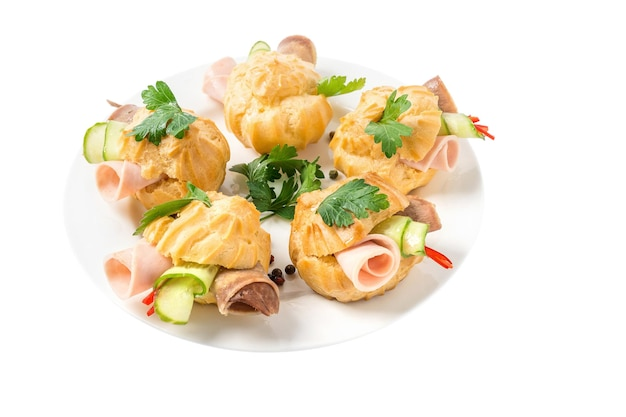
\includegraphics[width=7cm]{images/02_happens.jpg}
\end{center}

\textit{For years, potentially interested people have constantly been asking us and have wanted to know - and please in advance! - what actually happens at a Tantra seminar. We have finally surrendered to that request and are revealing it: Here they are, the facts!}

When you decide to be part of a Tantra group, it will be like all of you are being invited to a \textbf{big buffet}, with tables offering all kinds of delicious foods and snacks.

Some participants will wait until they got offered something three, four or even seven times, before they modestly go for it. Others will immediately jump for it, as if they haven't eaten for weeks. Some participants will look at the offer, full of desire and longing. Yet, out of fear of making a fool of themselves while using the snail tongs, they will stay with their good old mac'n'cheese. Others will shove heaps of potatoes on their plates and whisper to their neighbor how much they would have liked the salmon steak instead. Some participants will spend their time feeding others, instead of getting full themselves. Others will pick the raisins from the cake and then feel convinced they grasped the essence of the take. Others will stick to water and bread (which of course will also be served).

And everyone - really everyone - will find a range of learning opportunities: To find their personal right amount in the current moment; to allow oneself the carefree enjoyment; to say "yes" and "no" to all the offers; to have the courage to try something new, something unknown for once; to learn how to use these snake tongs in a playful way in a mutual trusting encounter; to try out life in its full diversity; to understand that there is enough for everyone; to understand that only a conscious celebration will bring deep and true joy -all of this, and much more.

At some point, you will drive home, your whole being still vibrating from all the unexpected new tastes and flavors. Regardless of whether it was one, three or five days: You will take enough momentum, energy and inspiration with you to recreate your own new menu of life.

\section{Surrendering - How does that work?}

\begin{center}

\includegraphics[width=6cm]{images/03_surrender.png}
\end{center}

For many people, it is still a test of courage to book a Tantra retreat: What happens there? What is expected from me? What if someone I know findsout about it? And even worse, what if someone I know will be there?!

Actually going there is already the first test of courage, and then taking the plunge yet another one. But what does it mean precisely, "to surrender" to such an experience?

It means to really make use of the offer (see the "buffet" analogy from the previous chapter), as it is indeed possible to visit a seminar for personal development without developing personally.

For example, I remember a psychologist, who literally sat the whole week at the edge of the scene. In each sharing session, he told everyone what "their topic" was. Or couples which do all the exercises exclusively with each other, sometimes adjusting them, and then feel puzzled why all the others report about all their new experiences and insights. Or participants who receive a call from a friend, their company or a parent right before an important exercise and only return to the seminar room after the exercise.

As you can see, it is easily possible to shoot oneself in the foot and deceive oneself in such an elegant way. Then one can avoid to be confronted with one's own fears, which only the others will be able to see.

The alternative, on the other hand, requires determination and courage: I need to want to experience who I really am, and how my inner world works, in order to overcome my inner resistances piece by piece. I need to be able to look the monster underneath my bed in its eyes, in order to be able to dispose of the harmless dust. I need to be vigorous to not simply stay stuck, although it might seem more comfortable at times, and to not give up on myself, even if I don’t know where to get the energy from to continue. I also must be ready to overcome too much pride and accept support and to realize when I am in need of it.

The good news: If you are consequently chasing after yourself, you will also find yourself. It even doesn't take too long! And what you will find is breathtaking and much bigger and more colorful than everything you were holding onto so tightly until then. If you were courageous enough to already participate in a Tantra retreat: Don't just put your little toe into the water! Jump in fully, with joy, and trust that the water will carry you. Because that thing you jump into is nothing unfamiliar at all.

That water is you.

\section{The rung ladder}

\begin{center}
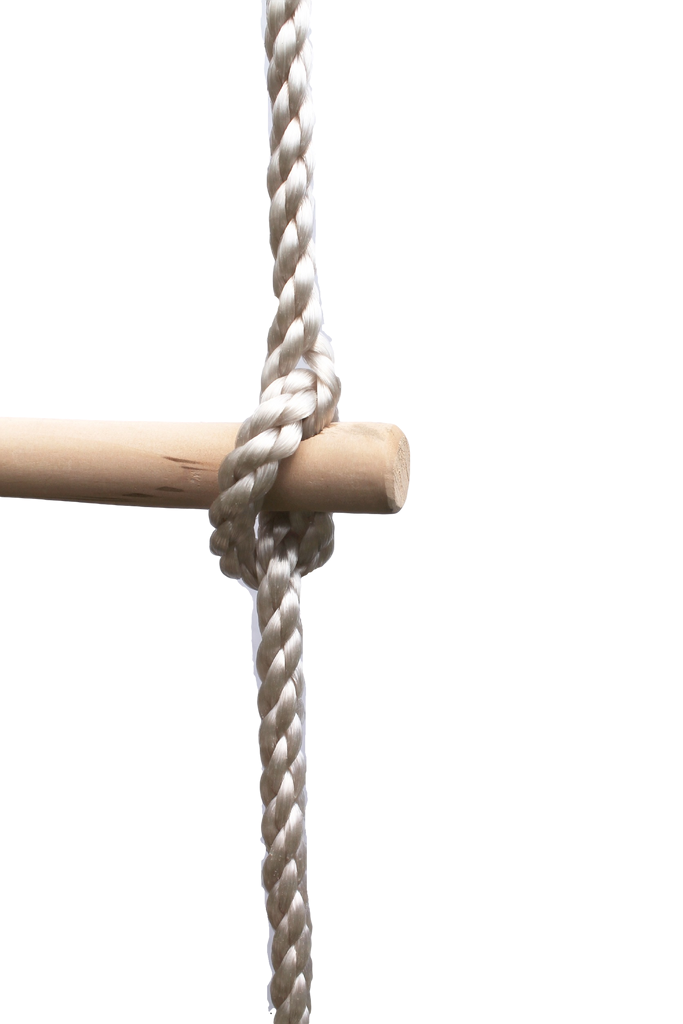
\includegraphics[width=2cm]{images/04_ladder.png}
\end{center}

\textit{"Tantra?! I already did that!"}

So you already dared to attend a try-out seminar and, chapeau, that took quite some courage! One does not know upfront what to expect, what kind of people will be there, whether the facilitators will be strange or guru-like, and of course: What about all these exercises? You have never ever done so much eye-gazing with strangers before, particularly not  at such an intensity. You have also never breathed so intensively, or at least not with such a firework-effect.

At the end you feel touched, showing your gratitude and telling everyone how great it was. Now you can check off Tantra in your internal to do list. Because now you know how it works, right?! And now you are able to contribute to the conversation when people talk about it.

Others from your seminar group, and maybe at some point also you, have the feeling that there must be more and continue. For example, you book a basic retreat. And wow! Although there are many things you recognize from the try-out, it is not comparable at all: You are more familiar with things, know your way around and feel home and cosy in the retreat setting. The simplest exercises have a more intense effect. You start to recognize your first patterns within yourself and others, which obviously make life more difficult, and receive tools to deal with them properly. At the end, everyone expresses their gratitude exuberantly.

Some of us know now exactly that they want to continue their search, and also others know with the same level of confidence that they received exactly as much as they wanted, "more is not needed". Their environment already asks them why they are somehow different, somehow in a better mood. Some of those who want to continue, to get to the bottom of things, consider a full year training. Yet others book the try-out event two, four or even five times  and report that it is new and fascinating each time.

A full year training tackles a bigger construction site: Here you look gently at old patterns, deepen your trust in yourself and the world, make peace with your body and make one or the other experience which you can't really express with words.

After that one year training you finally can relax, lean back, and know that you have mastered Tantra. What else should be there? Some of your seminar group might have a hunch that there must be more, that the actual essence is still ahead. The one year training might have been only something like primary school. And they continue... Those people, supported by the subsequent retreats for advanced participants, report their intention more broadly:

It is not only about the joy of life itself anymore, not about being happy, but about the ability to shape one's own life. It is about goals which go way beyond the ones of daily life and desires. It is more about how to live a life without irrational fears or how to see the essence of things.

Some will breathe lightly after the advanced training and be absolutely certain now they have learned everything that there is to be learned.

And the others? They will unswervingly continue to practice, in the 24/7 retreat of their regular, daily life.
\section{Light in dark rooms}

\begin{center}

\includegraphics[width=7cm]{images/05_light.png}
\end{center}

Some people come to us with the conviction that Tantra has something to do with spirituality. And they are damn right. Yet others are convinced Tantra has only to do with spirituality. And they are damn wrong. Often they already have spent some time on other paths which primarily focus on the spiritual component of being, and encounter Tantra along their way.

With Tantra, for a long time and especially at the very beginning, it is plainly about the body, the simple physical body: its needs which want to be understood and cared for, which has to eat and digest, which not always smells like roses and, with increasing age, shows uncomfortable defects. All of that seems to be contradictory to a spiritual goal: It is about the divine, the pure, the eternal, untouched by the earthly, whereas the material world is full of hardship, desire and sweat and constantly reminds us that everything which has a beginning also has an ending and dies. An insight which the human mind will accept only very reluctantly.

For many it seems wiser to focus on the higher, on the pure energetical. That means they meditate solely on the 6th and 7th chakra, on the sources of the ethereal and "let go of the bodily". And what is tempting about it: It works! At least for some time. One receives astonishing results indeed, visions appear, unforeseen spiritual spaces open up ... one has the feeling of finally having arrived.

If there still wouldn't be that bothersome lump, the body, which still has needs, producing less enlightened excretions, revenge itself with inflammation of the lungs if not protected properly and stubbornly has desire for desires. Many decide at this point to go against the body, denying it its needs until it finally gives up. Tantra goes in another direction.

It presumes that not the rich need financial support, but the poor ones. Not the spiritual needs to be freed - it was and has actually always been freed! - but the materialistically detained needs spiritual attention and transformation. Which refers to the body and everything which has to do with our dark, unbeloved aspects.

What good does it do to shine outside into a bright sunshiny day with a flashlight? How much more benefit does it bring to use this very same flashlight to (en)lighten all the dark, deep, less appreciated rooms of our own house, so that light and clarity find their way in.

It is indeed true that Tantra is focused on spirituality. But: It does not split off the body and its concerns with the material reality. The body is the temple in which the higher states happen, which makes them even possible in the first place. In order to get there, all layers of the bodily being need to be filled with light and recognition.

And that is exactly where Tantra leads you: It helps you to transform your body energetically so that it is not an unbeloved, materialistic appendix of the mind anymore, but an affectionately cultivated temple.

This way, you can go on adventures together with your body and soul, as a whole and undivided human being.

\section{What is Tantra?}

\begin{center}
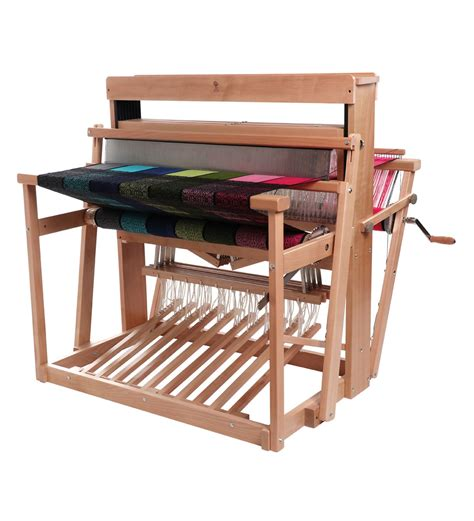
\includegraphics[width=7cm]{images/06_what.png}
\end{center}

\textit{The traditional Indian teaching can bring a fresh, erotic breeze into the bedroom, at least according to popular sexual advisors. Only few people know what Tantra is exactly about and what its actual purpose is. One thing is for sure though: Western Tantra can have a positive effect and be healing for every relationship in your life.}

So what is Tantra? This question pops up quite frequently. From people interested in spirituality, retreat participants, buddhistic practitioners and also from journalists.

The answer to that question can vary, as the topic itself is rather intractable, as it twists itself literally like the Kundalini snake and uncompromisingly requires an ever new approach.

Even the translation from the Sanskrit word \textit{Tantra} withdraws from a one-dimensional approach. Sanskrit dictionaries define the meaning of the syllables \textit{Tantra} like this: \textit{remedy, joy, loom, fire test, trick, oath, right approach}, and \textit{cause of more than one effect}. Other important meanings of \textit{Tantra} are \textit{scientific work} or \textit{religious discourse} (in reference to \textit{Tantra} as a designation for treatises from the Tantric Buddishm, such as Kalachakra-Tantra). Whereas in western culture, the word Tantra is understood as an umbrella term of methods for personal development, giving space to the non-hedonistic (not only pleasure focused) sexuality aspect of it.

These multiple meanings of the term often lead to misunderstandings among different Tantra practitioners. Many of the definitions are self-explanatory, yet I personally like the weaving, connecting aspect of the term the most. What exactly is being woven on the tantric loom and connected? Simply put: Opposites. They will be intentionally connected, until they dissolve and the boundaries are interwoven. Until the practitioner has catapulted herself to a space beyond duality and beyond the level of mental comprehension and, at least for some seconds, has reached her goal of pursuit. That's more easily said than done.

The dissolution of opposites, of contradictions, comes with massive inner resistances, as our mind has its difficulties to accept that there is something else beyond hot and cold, good and bad, existent and non-existent and especially that there should be something outside our mind. Tantric approaches always were revolutionary and created lots of resistance. That's also the reason why Tantra never became mainstream and why instead only a few seemingly half-insane people were concerned with it.
The early forms of Tantra arose about 4000 years ago in the south of India in the realms of Hinduism. Tantra radically stood against everything which was sacred to the older generation and which was considered the only true path of enlightenment: Strict purity, a cast system and a rigorous prohibition of meat and alcohol.

The disrespectful young generation claimed, on the other hand, that awakening will be  achieved exactly when worldly temptation will no longer be resisted with self-mortification. To the contrary: The temptation should be acted out fully in a sacral context in order to worship the gods, until its void, its meaninglessness, will simply reveal itself.

That might sound aloof or unreachable, yet something quite similar to that revelation can also be experienced in regular daily life: When, for example, after two hours of consuming social media, I slowly realize how mechanical, self-affirming and empty I feel after losing myself in this temptation.

Whoever wants to deal with unadulterated Tantra needs to bring a considerable amount of courage and lots of desire for change, because traditional Tantra still counts on provocation. Yet never for the sake of provocation itself but always to induce a fundamental change in one's thinking: To reach the realization of reality through temporarily turning off the conventional rules about this reality.
Some of those methods are surprisingly contemporary and psychologically well founded. Today, they can be found in texts such as the Hevajra-Tantra, which are the foundation for Sadhanas (practice texts) of the Anuttara-Yoga-Tantra.

What was valid back then is still valid today: for such an exceptional progress an exceptional amount of energy is necessary. It requires persistence while practicing, determination to continue, courage in difficult times, confidence when nothing seems to work out and the whole self-constructed structure of reality seems to break down. It especially requires wisdom and humility as strengths when at some point results from the practice show up.

But where should this huge amount of energy that is necessary to see reality for what it is come from? Where is that source, which is easily accessible, inexhaustible and holds irresistible powerful bubbles? The answer of the early Tantrics was obvious and still leaves people incredibly amazed : The force of creation. The power of creativity. The life force itself: Sexuality.

Tantra thus merges spirituality and sexuality and brings back the deep, mystical meaning to sexuality. Because what else could be more awe-inspiring than the potential to create new life? And nothing gets lost from this incredible awe-inspiring force if it is being used not for external, but for internal creation. This turbo boost enables us to experience this deep insight in a relatively short time. In contrast to what most usually think, Tantra never sees sexuality as a means of its own end. It is not about pleasure; that's only a comfortable side effect. Sexuality is just a medium, a vehicle, a form of meditation. Practitioners intentionally use it without creating a personal bond, to create enough energy and thus to quicker reach the goal of gaining a deeper understanding.

So if Tantra has nothing to do with sexuality as an expression of love and attachment towards a specific person, how is it related to relationships? Exactly: Not at all. Or at best maybe just as a side effect.

Yet again and contrary to what most people might think, Tantra is no exotic miraculous potion which helps worn-out relationships with Mantra singing, the smell of incense and acrobatic positions. If one understands Tantra in its traditional context, without turning it into  sex-gymnastics or couple therapy, then it becomes a practice for individuals which support each other along their path.
If we follow the hinduistic path, then - in a nutshell - one aims at liberating oneself from illusions. If our Tantra practice leans towards the buddhistic path, then we strive to contribute to the well-being of all beings.

Bearing all of the above in mind, are relationships in Tantra not an issue at all? Well yes, of course, if only a bit different than we are used to. One of the fundamental methods in Tantra is uniting contradictions. This can happen in the ritualistic union between the masculine and the feminine. Or it can be much simpler and ordinary. For example, by making it a daily practice to understand that everything (literally everything!) we perceive is a projection of our own mind, and the separation of me and not-me is just an illusion. No matter who I support, insult, admire or despise: It will always affect myself. That's why the dividing line between me and "the others", whether it might be based on nationality, income or attitudes, is just another illusion which keeps me imprisoned in a cage caused by an insane worldview.

Once I free myself from the chains of emotional and mental entanglement through practice, even just a bit, it will automatically affect all my relationships in a positive way. I will slowly stop blaming others for the discomfort in my life, understand the causes of their own entanglement better, and am more tolerant and patient with them. That would be a meaningful tantric exercise program in addition to a heightened consciousness, body awareness, a bright attitude and gratitude. Many think, however, that they already experienced Tantra by paying for a Tantra massage. Some couples also think that they have a "Tantric relationship", whereas they simply have an open relationship with changing sexual partners. In fact, polyamory only has something to do with Tantra marginally.
Whoever wants long-lasting Tantric joy and light-footedness in life has to invest quite some time and effort upfront. Authentic Tantra is not particularly consumer friendly. Instead it is rather effortful and not flattering for the ego if one is serious about the "get to know oneself" part. And that's exactly why we need these previously mentioned amounts of energy which we can very easily scoop from joyful, erotic activities. The catch here is that the original Tantra assumes that we have a natural, heartfelt and relaxed relationship with sexuality. If we have such a relationship, the bubbling sources of creative energy are truly available to us and we can cheerfully set out to discover all of it. Just who of us has a truly relaxed, neurosis-, stress- and embarrassment-free and joyful relationship with their sexuality? So in order to work with those sources of energy, we have to make them free and available first. That's why the so-called Western Tantra at it's beginner stage often resembles Biodanza and communication training, and at its intermediate stage it seems like body work, therapy and a school of life.

That way we train the body, mind and heart; gently, in stages and interconnectedly. The result is a holistic development of the whole human. Methods which ignore the body or even despise it are - from the point of view of Tantra - unfavorable, as without the body we would have no senses and therefore no sensual impressions. Without those impressions we would not be able to perceive the duality and consequently not transcend it.


\section{Teacher wanted}

\begin{center}

\includegraphics[width=7cm]{images/07_teacher.jpg}
\end{center}

\textit{How to find a good teacher.}

If someone is now curious about Tantra and wants to explore it, how do they  get started?

Learning it by simply studying a book is not only contradictory to its oral tradition, it is most probably also a waste of time, as most exercises can't be learned through written language. Especially during the first part of a Tantric path, a group is helpful. A group gives me the feeling of safety and supports me in seeing my potential for development. Along with that, having someone available who I trust, rely on and can ask questions helps me when in need in difficult times. As he or she has lots of Tantric experience of their own, this is a priceless support.

To find a proper teacher is a big project. One might think it should be easier these days, as in the past there was less offer and one had to travel very far in order to experience a retreat. Looking up the word "Tantra" in a search engine today, one is confronted with a flood of facilitators. This leaves lots of interested people clueless and they give up with frustration.

The following paragraphs contain a few indications which can but don't have to be regarded when looking for a trustworthy Tantra institution. If one doesn't find one, like me in my beginning, the lessons can also be fruitful, but far less enjoyable and the detours can be quite long.

\begin{itemize}
\item Finding the right teacher is special. Don't expect that it will work right from the beginning at the first attempt. Take your time, have patience. And yes, it may take years.
\item Which educational background does your future teacher have, what kind of qualifications? Is there proof for it? Do you know your teacher's teachers? If not, try to look them up on the internet. Go directly to the root source.
\item What does the internet tell you about your potential teacher? Don't be naive and don’t believe everything. Find facts, and carefully pay attention.
\item Are personal services and favors expected or even demanded, when you are in individual contact with the teacher?
\item Are common rules laid out transparently and are they comprehensible and challengeable?
\item Especially because Tantra works with sexual energy, it is of utmost importance to draw a clear line between teachers (including assistants) and students. Erotic innuendos, offers and requests coming from the teaching staff are a red flag. The same is true when teachers accept erotic offers from the students.
\item How does the teacher deal with his or her own weaknesses, flaws and mistakes? Is she able to admit to not knowing something, to be mistaken, or simply, which is very human, to have messed up something?
\item Does the teacher claim to be enlightened or to possess some special skills? Does he permit that others say similar things about him? What happens if doubt is expressed, or if he is critized in front of others?
\item Have a look at several teachers, within a retreat and also outside, in their "ordinary life". When they write books or articles, read them. Then make up your own mind.
\item Contact them personally. As long as you are not intrusive and stay respectful, a clear, friendly and in-time response to your questions should be possible. A guru figure, which is not even reachable via email, is of little help to students.
\item Have a close look at the teacher’s students, especially the advanced ones.. Are they good role models for you? Do you also want to think, talk and act like them?
\item What is the atmosphere in the group? How do they deal with tension, fears and resistances? Is there laughter, but not about others?
\item Check possibilities to opt out. It should be easily possible, at any time.
\item It is a good sign if your teacher motivates you to also have a look at other teachers.
\end{itemize}

You ticked all the checkboxes above, it looks promising and you have a good feeling about him or her? Then your journey can begin. A lot of joy and insights to you.

\section{Tantra: Beneficial for the backbone}

\begin{center}

\includegraphics[width=7cm]{images/08_backbone.jpg}
\end{center}

\ldots and with that, not only the bodily, moveable elements of a Tantra retreat are meant, which have astonishing, relaxing effects for many people! When you start to deal with Tantra, you usually have already gotten some life experience, enough in any case to have figured out that not everything on this planet runs smoothly: People get mobbed in the subway, contracts turn out to be a fraud, politicians are corrupt, relationships shatter, intrigues take place in the office and your best friends cheats on you.

Now there are many ways to deal with these depressing facts: One can duck one's head and pretend that nothing is happening and hope it will pass soon. One can shrug one's shoulders, sighing that the world is simply ruined. Or one can stand up and do what needs to be done. That's what's called moral courage, which is not very attractive, as who wants to expose oneself?! To speak up and probably get a slap for it? Who wants to get in trouble with the ones who are in power, like the daring activists have been doing? To do it nevertheless requires a lot of courage and the same amount of wisdom, because without wisdom, courage is just crazy foolhardiness, and wisdom without courage only sits uselessly behind the oven.

And what does all of this have to do with Tantra? Tantra, in the way we understand it, has only peripherally to do with sexuality. It is more concerned with getting to know oneself as well as possible. People who know themselves better estimate their potential more realistically. That's how they are able to keep standing up straight, even if others try to make them small. That requires a spine, and that spine is not given to us at birth, but we have to acquire it through hard work.

And how does that work? By getting out of our comfort zone, into unfamiliar, challenging situations and, with the support of others, master them. Because fear starts to dissolve when we don't avoid it, but kindly approach it and finally embrace it. We gain a backbone not only with our body and mind, but at the same time by training our courage, compassion and serenity. For example with Tantra.

\section{Is Tantra dangerous?}

\begin{center}

\includegraphics[width=7cm]{images/09_dangerous.jpg}
\end{center}

Whoever gets involved with Tantra is searching for something. How do we know that? Very easily: For the sake of using up time there are plenty of activities which are considerably less time-consuming, less effortful in energy, courage and patience than Tantra.

So what is the goal of this search? One thing that moves the most in the deepest way is the search for meaning, especially when in their personal history painful experiences  have happened. The search for making meaning of such experiences as well as of life itself can only be successful if we enlighten our dark spots, hidden in the shadows. If we bring light to those almost forgotten and carefully suppressed painful experiences.

That might not always feel like a stroll through a rose garden, which lies in the nature of things, and thus we can confidently agree here: Yes, Tantra is dangerous, as it endangers your whole past view on the world!

I remember a participant about the age of sixty. She took part in a short entry-level retreat and courageously stayed until the very end, even though she obviously had to struggle with intense emotions. Afterwards she came to me and said: "You know, it's all nice and good here, but I think I would rather not wake up those sleeping dogs."

That's a valid and conscious decision: I prefer to keep my view on things. The effort to gain a new, probably more relaxed worldview is too scary for me for now. Yet, once you have determined to bring up the light out of the depth, then it is rather irrelevant what you do. You can even attend a plain painting course: Something you experience there will bring the burdensome experience from the past to the surface of your consciousness, so it can be dissolved.

That's also what Western Tantra does, just with caution and focus and with the support of thoroughly and extensively educated facilitators.

Does it also happen that someone seriously "freaks out" - due to an intense contact with an emotional burden of the past - and is not able to help himself or herself anymore? Indeed, it does. No effective method can guarantee harmlessness. But we had to intercept such a situation only a few times within the last 25 years. For such moments, good facilitators offer competent and empathetic support in the process, during the retreat and also afterwards if requested.

Tantra uses an approach which carefully reveals old and deeply hidden things.That's why there is so much astonishing feedback of therapy-experienced participants. They cannot believe that even after a single retreat they have progressed so much more than in many years of conventional therapy. However, their previous effort is never in vain. Often it is exactly due to a past therapy that they can get unexpected and quick results.

To sum it up, is Tantra  dangerous? Absolutely!

Your destructive thought convictions, rigid patterns, less than helpful habits and all the other elements which prevent you from reaching your highest potential may already be scared.

\section{Hard work or celebration?}

\begin{center}
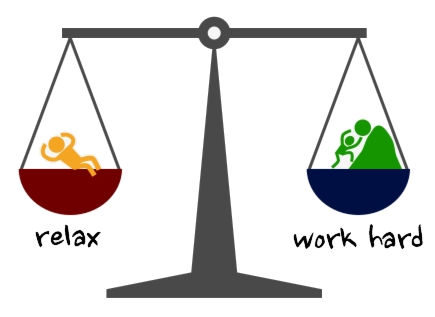
\includegraphics[width=7cm]{images/10_work.png}
\end{center}

"Well such a retreat is hard work, that can't be denied. It starts with getting up that early. Do the meditations really have to take place at 7:30 am every day? And also, why is she so peculiar about us being on time? Come on, we are not in school here! I thought we were supposed to learn to enjoy life in the now? To comply with all those rules is pretty tedious, that's more like work.

Wow, and everything is so structured: No water bottles are allowed in the room! And I am supposed to share something meaningful about me in front of all the others in the sharing circle before noon! Dancing - me?! Oh well, and then the program that lasts until late at night, are there no considerations for morning grouches?

And that was just the beginning. Then there are those exercises. To eye-gazing with total strangers, and that already at the try-out seminar. Breathe, as if there was no tomorrow. And then I am supposed to doeverything consciously... teeeedious!

It gets especially hard when we do exercises which are not that easy for me. Constantly overcoming these obstacles and motivating myself is tough work, no question."

"Hard work?! Well, only if one also refers to an adventure holiday as work.

Being on time is not a big deal as your curiosity and the excitement drive you: What might they have planned for us today? What are they going to surprise and challenge us with? Where will I learn new aspects about me? Where will I encounter limits or finally break out of an old, much too small snail house?

And the dancing! Only flying is more beautiful. Everyone on their own, all together, looks are so irrelevant! What is important is that you are allowed to show yourself, the way you are right now. Crazy, shy, stubborn, blissful. Everything is welcome. Where else do you find that?

Oh, and the sharing circles... Very impressive, touching, so much openness, vulnerability and to be given so much trust. To find oneself in the others.

In the breaks, we continue with long conversations. Deep, good talks, which bring my life on new tracks. And not to forget the touch and breath exercises. Pure bliss, timeless, vibrant energy. Unintentional, pure joy!

And by the way, the 'work' really pays off: Also my environment realizes that something is different about me, because I am simply in a better mood. I recently even spent a whole week at my parents' place. And you wouldn't believe it: They were almost unrecognizable to me!"

\section{Mindfulness: A short introduction}

\begin{center}
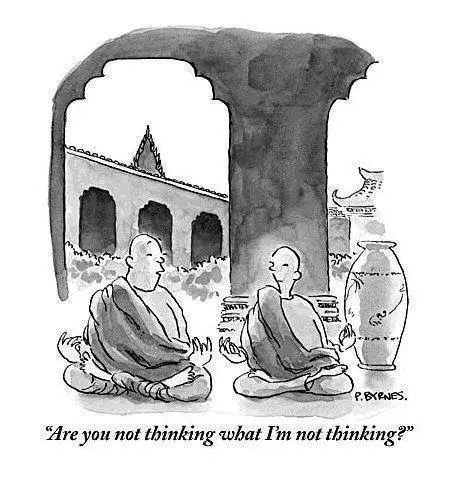
\includegraphics[width=7cm]{images/11_mindfulness.png}
\end{center}

\begin{leftindent}

A (\textit{sits in a perfect lotus seated position and looks to B in a requesting way})

B (\textit{sighs deeply and tries hard to somehow sit comfortably on the pillow without falling down or dislocating his hip})

A (\textit{closes the eyes with relish and takes a deep breath})

B (\textit{tries hard to keep up and takes a deep breath as well; which sounds more like a groan})

A (\textit{unctuous}): So? What do you feel?

B (\textit{opens the eyes; slightly in panic}): Feel? What should I feel?

A (\textit{gently}): Whatever is right now. What is right now?

B (\textit{confused}): What should be right now?

A (\textit{with godly patience}): What's in your body? What's in your thoughts? What kind of emotions are there?

B (\textit{completely overwhelmed}): Hmpf...

A (\textit{turns a gear down}): Can you feel your body?

B (\textit{clueless}): No.

A (\textit{still very patient}): ... your hands, the way they rest on your knees?

B (\textit{delighted}): Yes!

A (\textit{relieved}): Look, it's doable. And what's happening with your feelings?

B (\textit{suspiciously}): Which feelings?

A (\textit{pushy}): Well, the feelings you have right now.

B (\textit{categorically}): I don't have such a thing.
\end{leftindent}

\vspace{0.2cm}

Mindfulness is good and important, it lowers the blood pressure, makes a leader out of you, results in stable relationships, catapults you to enlightenment and much more. Everyone is practicing mindfulness these days!

To practice it, like we also do at Tantra retreats, is indeed required, because sometimes we don't know exactly what is meant with "being aware": Do I have to focus very strongly? On what exactly? How do I recognize that I am mindful right now?

Mindfulness training begins with something simple, something we always have with us in any case, and with which we are kind of familiar: our body: You can sit upright, maybe close your eyes, and feel whether you can sense something. For the beginning, that can be your breath or your heart beat. In case that works well already, you can be aware of warmth or coldness in different parts of your body, a tingling, a pull, tension, movement or pressure. With continuous practice more and more subtle sensations will emerge and you will be able to recognize reactions on impulses based on small body signals, like a small shivering, dizziness or a grumbling in your belly. This impulse can be something external, like the temperature or the words of someone else. It can also be something internal, like a thought or a feeling.

To turn one's attention to those impulses without judging them, clinging to them or turning into them is the key to many goodies, which mindfulness brings us over time. For example, a merry and unshakable serenity in daily life.

\section{Jealousy}

\begin{center}

\includegraphics[width=7cm]{images/12_jealousy.png}
\end{center}

\textit{Believing that jealousy has something to do with love is a misconception.}

"The more you love someone, the more jealously you react", "Jealousy is proof of love" - we have been hearing such statements ever since we were kids: Cheap novels want to convince us and pop songs drool those kind of lyrics upon us.

Truth be told, it is more like this seemingly superficial German saying states: "\textit{Eifersucht ist eine Leidenschaft, die mit Eifer sucht, was Leiden schafft}" (jealousy is a passion, which seeks with eagerness, what creates suffering). Take, for example, when we justbroke up with our partner, and that partner then gets engaged with another person. Or: It doesn't seem like a big thing for you to have a side-relationship, but if your partner claims to have the same right, you get indignant.

In the name of love, which is supposedly the source of jealousy, we beat others verbally and physically. When one suffers, the other will be made to suffer too. Threats, blackmailing, torture and homicide can follow. There are still countries where the so-called "murder out of passion" is still free of persecution (of course only for men). Does this look like love?

When we have a close look at the impactful effects of jealousy, we quickly can identify its roots: Violence has two main sources: the claim to power and fear. (Even if violence is expressed very mildly through punishment by sulking or dramatically by making a scene, threats or physical violence, or even against the one who is jealous himself, reaching from "I haven't deserved it any better" to suicide).The power claim is based on the conviction that one has the right to decide over the lifestyle of the other, or at least have a big influence on it. This self-proclaimed right is based on the belief that the other person "belongs to oneself".

Today we are all too well educated to speak out such things loudly. However, the imprints of past centuries and millennia still have a relentless, hidden influence on us. We feel those painfully when we get in contact with geographically more remote cultural conceptions, that are getting more tangible now.

There is this fear to lose that power, on the one hand, and to be not good enough on the other.  The fear of competing, of getting uncomfortable, of letting go of safety and of confronting oneself with a novel situation. Of being forced to let go of territory, or of consenting to new, less comforting agreements for the ego.

The combination of a claim to power and fear is highly explosive, and shows itself on the surface as anger and revenge ("\textit{What?! You hurt me?! Just wait, I'll show you!}") or also as victimization ("\textit{I will never be able to trust someone again}") and leads to those kind of discharges which are well known in scenes of jealousy.

In order to throw a devastating punch at our former beloved one and now deadly enemy, no big words are necessary, as often a small glance is sufficient to destroy what has been built up over a long period of time. So what do we do in such a specific case, so that the jealousy bomb won't blow up?

\begin{enumerate}
\item First of all, you have to admit that you are jealous, because the ego likes to conceal it behind justified anger, fake indifference,...
\item Furthermore, you have to be clear that jealousy doesn't lead to any constructive results for anyone: It can only destroy, persistently.
\item Next step: Try to reason what's behind the jealousy. Do I identify myself through my partner and am I scared to disappear once my partner is not there anymore for me? Am I outraged because someone entered my territory? Do I feel insecure because the other one is younger, knows better how to deal with computers, ...? Do I actually want to hide and cry, because I am panicking over change?
\item Communication. Very often, being jealous lacks any real foundation (this also relates to the German saying at the beginning of this chapter): Maybe the other person was her cousin? Maybe she just enjoyed the flirtatious eye contact with the waiter because he made her feel reassured about  her femininity -and that's it?
\item Tell the other person what's happening inside of you. Start the sentence with "I ...", as in: "I am terribly mad because I have the feeling that ...", or "I am totally insecure because ...", or "I have a problem with ...". Avoid generalizations like: \textit{ever, never, always, a hundred times}.
\item If it is impossible to talk about this topic without overwhelming emotions, ask a person whom you both trust to join you. Just their presence can smoothen the emotional waves. It is a sign of maturity to ask for professional help when in need.
\item And yet again: Talk with each other!
\item If that is currently not possible at all: Be silent with each other. Keep eye contact for about 20 minutes and let the eyes do the talk.
\item Let the bodies also do the talking. The body often wants something totally different than the scared heart or the confused head. Touching each other’s hands and communicating with the fingertips can be a stunning and utterly reconciling experience.
\item If there has not happened anything seriously bad yet, and the deeply injured ego can let it happen: Sleep with each other. In case your despite is insurmountable, be aware that you don't deceive yourself. From a certain perspective, you are not surrendering to your partner, but always to love itself, your own love!
\end{enumerate}

A sexual encounter, which is rooted in love and happens for that love, and that is not abused to pressure someone, is a powerful medicine and can lead you two to the point where you both know what you mean to each other. Regardless of how strong the wind howls outside.

\section{One's weaker self}

\begin{center}
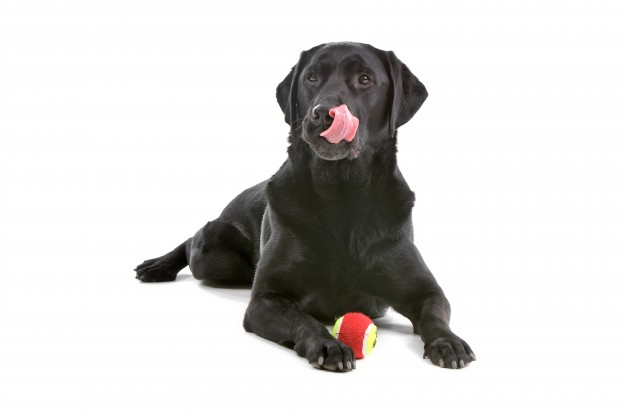
\includegraphics[width=8cm]{images/13_weak.jpg}
\end{center}

\textit{I do want to do the right thing, but how?}

We all want to do the right thing. No one wants to upset another person. Most of us believe in the actual good within each other, and so also within ourselves. Yet, we often do what we afterwards regret and feel ashamed of: We speak words that hurt others; we do not reach out our hand although we know it would be the right thing to do; we take what we want at the expense of others and find justifications why it is our right to do so.

We react in a snotty, sulky, rude, sarcastic, jealous way or like a smartass. We feel threatened and think we constantly have to defend ourselves against attacks. And we break our promises, towards others but especially towards ourselves. Just think about new year’s resolutions.

While our weaker self, this little lazy dog, runs its circles on an extremely long leash, everyone also has another part within themselves: A part which is pure, innocent, free of intention, and full of confidence and trust. So how can we evade that lazy dog and let that other part take control of the steering wheel? How can this gentle little thing outshine this loud barking dog inside of us?

The answer is simple and also, at the same time, uncomfortable:

First, we have to train that dog, so that it won't move around wildly anymore, but sit still and give us its paw. That requires some work, which in Tantric Buddhism is called "to tame the spirit". This kind of work is challenging and tedious, as the weaker self speaks in the exact same voice as the higher self does, and to be able to differentiate those two takes a lot of time.

Furthermore, we have to bring this breathtakingly beautiful, yet also very vulnerable part of us out of the protection of the darkness and make it visible.

Isn't it endangered through that? Yes, it is. Can we be hurt when we show ourselves vulnerably? Yes, we can. Will we be taken advantage of immediately and sucked empty and fall victim to sharks? Most likely not. Because that tender part of us is not totally helpless and whiny. It also doesn't blame others when something goes wrong. It is full of wonder, compassion, generosity and joy, which doesn't need a cause, and love, which doesn't ask questions. And that part is also courageous: While the weaker self (also called the "ego") turns away and mumbles "this is not my concern", the tender part (let's call it the "self") does the right thing instead: It apologizes, remains silent instead of quarrelling, and hugs instead of bitching around.

Because we know exactly what's the right thing to do. We just have to learn how to differentiate those two damn voices from each other.

\section{The only true teacher}

\begin{center}

\includegraphics[width=7cm]{images/14_teacher.png}
\end{center}

We regularly receive emails from people who explicitly ask for a specific facilitator and sometimes add: "If X or Y isn't going to facilitate, then I won't come... Because s/he is so great, and I don't know the others from the team and I'm also not interested in them."

Well, to participate in an event that is very much about getting to know oneself, doing bodywork and also about healing the so often crushed sexuality, definitely requires trust. Without reasonable trust in the facilitator, many would be constantly on guard to protect themselves. This way, the gains from such an event could be rather small.

That's why as a participant, of course you make sure that you can trust those who instruct the exercises and play the music. This trust grows with subsequent events, through direct conservations and questions. Also single practice evenings and other short events are a good possibility to verify and deepen your trust.

Of course you will have your personal preferences among the teachers, just the way I did, at least at the beginning, and just the way I had my preferred exercise partners. But this should not be the final state of the development which we guide in retreats. Because if everything goes as expected, at the end you should be more and more indifferent (German: "\textit{gleich-gültig}", lit. "same-valid") with whom you do the exercises. Then I know, based on all the experience I already gained, that I do the exercises first and foremost for myself, to get to know something about me. My exercise partner is an essential help and therefore very welcome, yet, s/he has less and less influence over time on whether it will be a "good" or a "difficult" exercise for me.

Advanced participants have gloriously reported that they can now do any exercise with literally everyone from the group in a relaxed and joyful way, regardless of whether they are well known or strangers.

A similar situation can be seen with the facilitators: If everything goes to plan, you can slowly let them go. Their roles as substitute parents and projection surfaces that were natural and important at the beginning can now be put behind. Now the responsibility for personal happiness and well-being, your very own safety and the trust in oneself and the world is not passed over to someone "up there", but gradually taken over by oneself. And that's exactly how it is supposed to be.

The goal of a good facilitation team can't be to be adored, applauded to and to be used. To the contrary: The goal should be to put oneself as a facilitator more and more into the background and to become more and more superfluous. Even to a degree  that the participants only vaguely notice that there is someone at the front and instructs, while they relax and confidently sink into the exercises and experience.

\section{Protect yourself}

\begin{center}
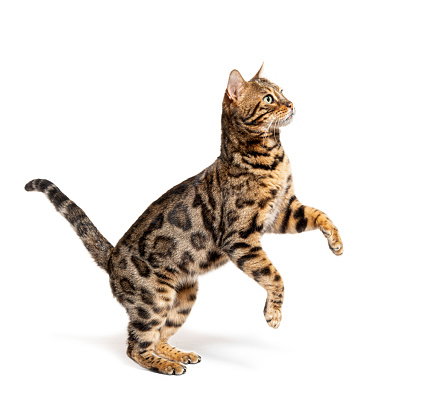
\includegraphics[width=6cm]{images/15_protect.jpg}
\end{center}

\begin{textit}
Should we protect ourselves? And from what?

My cat sits on the windowsill. It's about two meters to the top book shelf that he wants to jump on. He takes aim.

He evaluates.

He checks out different points of view.

He wriggles on his spot.

Then he vigorously jumps... and lands.

Elegantly.
\end{textit}

A participant explains to me that she cannot come to the practice evenings because there are always these "intense energies and she needs to protect herself from them".

I don't say anything.

It is not the right moment to reasonably ask whether some "other" energies are really "out there", or if it might be a product of our own perception of the mind. If I assume that there are monsters underneath my bed, I will also find them there.

I myself don't believe that I have to protect myself, at least not beyond a reasonable amount, which prevents me from being hit by the very first truck on the street. Of course I too am afraid sometimes. I too have read the news, have my childhood traumas, went through quite a few unfortunate experiences and huge disappointments and know roughly what can happen in life.

But to protect myself by not exposing myself to life and its challenges, surprises and contradictions would mean that, in fact,  I cut myself off from my own (!) life. And that would be even worse than what possibly could happen.

Yes, to encounter people can be exhausting. And it is true that executing tasks can lead to frustration. We can also agree that saying yes or no to the other person can lead to rejection. No matter what I do, I expose myself to the danger that something can go wrong. Of course we want to safeguard ourselves from that, to protect ourselves! We can achieve that by retreating into a safe cave, or \ldots

\ldots or we can protect ourselves by encountering those scary experiences with open eyes and open arms, embracing them.

Should we evaluate the situation? Of course!

Should we strive for the best solution? For sure!

Should we think thoroughly, to give myself advice? Hell yes!

But then jump vigorously!

Like the cat.

Because the fear of life and the need to protect myself from all those scary things can only be discarded by having trust in life and myself. And that is only achievable by doing precisely those things I feel a bit scared of.

\section{Just married + Tantra}

\begin{center}

\includegraphics[width=11cm]{images/16_married.jpg}
\end{center}

\textit{How do Tantra retreats work when you are married?}

That frequently asked question shows that for many married participants this is a contradiction in itself. And they are right. Although, only if you assume that Tantra means living out pubescent desires for endless sex without commitment, responsibility and connection.

If you think, on the other hand, that first you have to get rid of the skeletons in your closet in order to start and maintain a happy relationship, things start to look very different.

Additionally, if you wisely choose a partner who rarely projects his own childhood traumas onto you and mostly  copes with his emotions, needs, fears and frustrations - just like you -  the chances rise considerably for a love which is "free" in its wider definition. Free not of commitment and responsibility, but free of neurosis and childish projections.

If this is paired with the insight that relationships are a life long learning process, with oneself, with the other, and with each other, that there is no higher level of Yoga than marriage. Then we don't simply throw away everything and look for "something better" just because things escalate every once and then (Heaven can be full of trumpets instead of violins sometimes.). And we realize that our happiness is not our partner's but our very own responsibility. Then the combination of married and participating in tantric retreats for personal development is absolutely plausible. 

In order to experience, explore and understand ourselves as whole human beings, we also have to carefully deal with aspects of sexuality. A small part of Tantra deals with this topic. This exploration can be done in exercises, meditations and reflections, alone or together with others. It is not really surprising that as a couple, one will be faced with fears of not being good enough and abandonment. This contact with one's own personal fears doesn't need to be followed by a jealousy scene: If I can love pretty free of neurosis, then I am also pretty free of the obsessive need to "own" my partner  exclusively, permanently and forever, or at least for how long it suits me.

We accompany many couples who go on an exploration together but also separately, sometimes joining the same retreat, sometimes alternating. It is encouraging what they have to report: They mention unisono the growing closeness, emotional safety, re-established bond and deepened intimacy.

Awakened love does not want to own the other, but to see the other happy. That's why long-term relationships are such an inexhaustible source for tantric practice. Much more than just exhilarating, erotic togetherness.

\section{The rusty screw}

\begin{center}
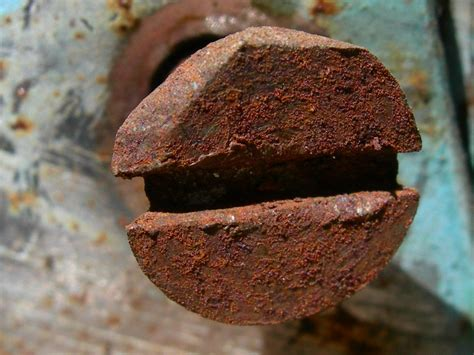
\includegraphics[width=7cm]{images/17_screw.jpg}
\end{center}

\textit{What does Tantra have to do with sex again?}

We are not mainstream and most Tantra schools put their emphasis on other topics. It's not good for business: after all, sex sells. It is not even easy to comprehend for many as "Tantra has much to do with closeness, touch, intimacy, thus sex, right?!"

It's irritating for those who have shown off their joy for desire like a hip accessory which states "Tantra". And now it is gone! Quickly it is not simply about the joy of lust anymore, but it is more noble sounding and close to enlightenment. It is not that joyful anymore, but instead the flawless strive for universal unity reveals itself.

We say it again, and we will say it every time: \textbf{Tantra only has to do with sex marginally}.

There is nothing wrong with pure lust and joyful fuckery is nice. But it is not the goal of Tantra. So why do we deal with the body, feelings, energies, exploration, discovery and the healing of our sexuality at retreats anyhow, if it is supposed to have nothing to do with Tantra? Because Tantra uses the most original of all energies, in order to develop mindfulness, insight, patience and the slow detachment of the ego. This primordial energy is available within us in huge amounts, and we can tap into it the most easily through joy which we experience with increasing erotic tension.

Most of us have no unbiased access to this energy source due to upbringing, social imprint, personal history, \ldots That's why Western Tantra aims at smoothing out the deformations in this area during the first stages: Fears, trauma, role models, prejudgements, \ldots

The exercises which are being offered are not means to their own end, and if you succeed in an exercise, you are not there yet, you haven’t reached the goal, because the goal of Tantra is not an easy going attitude to sexuality. An easy going attitude to sexuality is rather the precondition for Tantra.

The exercises at a retreat are more like supporting wheels, just like young kids use them when they want to learn how to ride a bicycle: Once they feel safe enough to sit in the saddle by themselves, they don't need the supporting wheels anymore. The same applies here: Once the goal of total insight is achieved, the exercises become unnecessary.

Just take, for example, a rusty screw, which is mounted wrongly and wobbly, and can do its job only half-heartedly. In order for it to be mounted properly again, we first need to free it from the rust. That can be effortful and take a long time. Yet, only few will think that cleaning off the rust is the actual goal. At the end, it is about the screw itself and as soon as the rust is gone, it can be screwed in nicely again and we stop cleaning it.

Thus, in Tantra it is not about a better, more amazing, exciting, \ldots sexuality. It is about making this primary, creative, potent energy accessible (with lots of discipline, by the way) and about using it as a vehicle to achieve the actual Tantric goals: Ever deepened awareness, mindfulness, loving kindness and serenity in every situation.

\section{The illusion of being separated}

\begin{center}

\includegraphics[width=4cm]{images/18_separated.png}
\end{center}

(\textit{or in German: "ge-trennt-sein", as in "to-cut-being"})

At the very beginning we know exactly: We are the world. The world is us. And the world is dark, warm, chuckles quietly and swings us gently.

As soon as we are roughly six months old, we slowly start to understand: That's me, and that's the others, and around us is the world. And we are proud of it, and so is our environment.

We eagerly develop and grow with that very same eagerness into this perspective, that on the one side there is us, and on the other the rest of the world. By that time, the rest of the world expresses itself with a considerable amount of unkindness, by taking away our teddy bear and not giving us the bike of our dreams. And out of incomprehensible reasons (too cold?! WTF?!) it does not allow us to get some ice cream, but expects us to do our homework.

We grow older and realize: The others are different. Some walk around veiled, some exclusively eat organic whole seed bread for lunch. Others claim girls can't do math, and yet others tell on their presumably best friend.

Fortunately, we know exactly what's the right thing to do, because we learned that from mum and dad. Accordingly, we know that anything that diverts from this is wrong. And our thin line of separation becomes a huge gap. Which also has its advantages: As we have absolutely nothing to do with the outside world, we can perfectly blame it for all the misery that happens to us.

For example, that annoying neighbor's dog, which barks loudly and endlessly, and is the reason why we can't study and already failed our exam for the fifth time now. Or that stupid cop, who takes away our newly gained driver license, only because we drank just a little bit of alcohol. Or that bitch from across the street, who took away our guy. Otherwise, he surely would have stayed with us forever. Or the government, the weather, the school system, the moms, who are to blame for everything anyway.
So it's not really that uncomfortable on this side of the gap between us and the world. Unfortunately, those who are to blame now have the power in their hands, so we are left with a lifelong, outraging and resigning nagging about our helplessness in this hopeless, separated world. And then there is this thing called Tantra.

Tantra tells us unconscionable things like: \textit{Look around. Everything you see is you. That's your world, your universe, created by yourself, shaped by yourself. Anywhere you look - everything is you!}

If you do not immediately fall unconscious due to this vile insinuation (\textit{What, even the wars? The stubborn non-vegans? The stranded whales and cut down rainforests, the doubtful politicians, my terrible job and that neighbor's noisy lawn mower?! Everything is me?}), you are invited to try it out: Look around and think about everything you see in the following way: "\textit{That's me, and that also...}". No, don't just try it soon-ish. Do it now! Exceptions are only valid for confirmed coma patients.

Whatever annoys me, irritates me, makes me sick or angry: It is part of me. Whatever I groundlessly admire: It is part of me. And that's why I can't (ha!) be generous, mild, kind or patient … enough, because I'm all of it for myself!

As it is suddenly no one else's fault, I can start to take things in my own hands... and the gap between us and the world starts to dissolve, until we finally end up where we originated: We are the world.


\section{Maithuna - An experience}

\begin{center}

\includegraphics[width=7cm]{images/19_maithuna.png}
\end{center}

Maithuna.

\textit{"Finally free sex, some say, and it even has a spiritual cover on top of it! Tedious, others say. Who should be able to sit upright for so long? Maithuna! That's the thing with the different positions, isn't it?"}, some ask.

Oh... Maithuna... that's not for me. Everyone has to interact with everyone, and it takes forever. Where's the fun in that, others moan, but not out of bliss.

Maithuna means union, and that refers to all levels. It encompasses the body and the mind and points out a path out of the daily entanglements of the duality: To be willing to be one with all that is.

\textit{With all that is} entails emotions, hopes and also deeply embedded personality patterns, as well as physical pleasures such as desire, suffering (for example pain in my knee) and the magnificent, annoying, unnoticeable presence of my partner.

To try to explain what Maithuna is, without having experienced it first, inevitably has to fail. One cannot describe precisely the taste of an unknown fruit. And still there are moments where one tries to do the impossible, even if one knows better.

In 2013, during a Maithuna ritual of one of our more advanced groups, I became a witness of such moments. I couldn't resist writing down what I saw and astonishingly observed what was unfolding right in front of my eyes, in this silent room beyond time. I almost didn’t dare to breathe in order not to disturb this perfectly smooth surface of being. There was something going on that I couldn't put my finger on, and yet desired so much to hold on to: Permanently, like when drawing a heart on a window that one has breathed on.

When I wrote my PhD thesis one year later, I wanted to use this text at the beginning as my introduction. But I didn’t do it in the end. It was too intimate, and only few would have understood it. Maybe, just maybe, here is the right place to put it.

The sun is shining through the uncovered window, drawing a moving pattern of time on the honey-yellow wooden floor. Eighteen candles are distributed in the room. Everyone is placed next to another person. Groups of three or four sit next to comfortable mats. Every perceivable movement happens with attentiveness, just like in slow motion. Carefully picked music supports their inner and outer rhythm. There are quiet touches, mindful hands and open glances. Unconditional presence which doesn't need words is in the room. I hear laughter, sighs and cosy purrs. I see pairs of eyes which close and then melt into each other again. No need to rush, no goal is noticeable. Everything unfolds in a natural flow, as if time has stopped.

Later they will be asked how many hours they stayed in this state. Or, maybe even more likely, they will not be asked at all.

If anyone of them encounters inner obstacles, everyone knows that there won't be any attempts for rescue. Everyone is responsible for themselves and is a competent expert about their own needs.
Sometimes someone loses himself in a maze of his own resistances of wanting and not wanting. Then everyone trusts that he will find his path back to himself, in his own time. But they also don't give up on someone who is temporarily confused: They stay attentive, open hearted and relaxed. They don't take responsibility for each other, but keep their doors loyally open for each other.

The men don't have to prove anything. They have learned to follow the flow of the moment and to trust their body and mind. What is, is. What isn't, is not. There is nothing to correct.

The women neither show stress nor bias. They obviously feel good in their bodies, regardless of their appearance. Everyone is present in their very own sovereignty.

Sometimes there are moments of complete stillness, sometimes there is a firework of energy, giggles and hearty laughter, sometimes there are tears. The participants don't talk, except for the ritualising formulas.

Meditative states interchange with outbreaks of spraying ease. Minutes, or rather hours, of silent immersion, together or alone, merge in roaring waves of highly energetic interaction. Playful and always discovering things from scratch, they feel joy about all the innocence and sensations which are provided by their wonder-ful bodies. Later on, they will report about deep insights, the shimmering kaleidoscope of new emotions and behavioral patterns, which they could observe in themselves. What a liberating understanding to be transferred to daily life!

But in this moment, they seem to be totally in love and intimately connected with their randomly assigned partner. And while they are on the mat and the ritual lasts, they are indeed in love, united with themselves and the universe, sighing, laughing, crying and falling silent in astonishment.
The picture which reveals itself in this room is amazingly intimate, mysterious, and touching eternity, so I almost don't dare to look.

Something like this, I can imagine, is how awakening looks like.

\section{Is everything sunshine, if I simply want it?}

\begin{center}
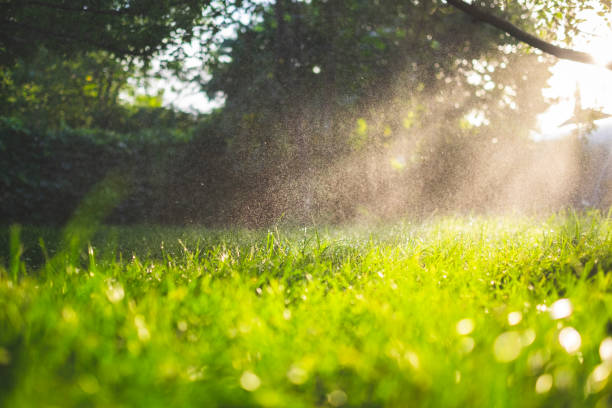
\includegraphics[width=5cm]{images/20_sunshine.jpg}
\end{center}

Whoever believes that sunshine can be created by simply visualising it is naive, or has let themselves be convinced by toxic positive-thinkers. Sunshine can't be wished from existence. Sunshine either is, or it isn't. Right...?!

When my child is sick, or my husband feels attracted to another woman, when my neighbour plays Heavy Metal at two o'clock in the morning, or when I'm in sheer panic of going to that meeting tomorrow at work, it is of little value to convince myself that everything is completely different than it is. Also physical pain, let's say sciatica, can only be made to disappear (through meditation, breathing) by only very few.

Common people like us rely on being somehow able to deal gracefully with the lack of sunshine in one way or the other. That's not easy, but it's possible. An important tool is to be able to learn to love the rain.

"Great", you say, "I shall rejoice, even though my child has the measles and I have absolutely no clue what I should say at tomorrow's meeting?!" No, you do not necessarily have to do this with rejoice. Only... let's say, reduce the resistance a bit, so that there is some space to breathe. Because resistance is fear, and fear tightens you up, and when it gets tight, breathing is more difficult... and when we can't breathe properly, we neither can think straight nor feel sensitively.

Even the most sophisticated form of resistance will change absolutely nothing about the current facts, but simply use up all your energy until exhaustion. So just have a little bit less of it, ok? Good! Now we can finally breathe properly again. Aaaah. Rain is good for the environment. Measles is good for...? Ok, here is a list: Measles is good for staying at home with the little ones. For developing a deeper connection between us, while I swipe away the hair out of their faces. For reading to them from a book, which has been overdue for a long time. For the inspiration from this story for tomorrow's meeting (dragons can be friendly, too!). For those breathtaking 10 minutes of silence when she finally falls asleep. For this crazy (German: "ver-rückt", which literally means “shifted”) feeling of calmness in the eye of the tornado. Is this sunshine? Most probably not.

But it's a good, rich rain. One which washes away so much which has been dusty for so long. One to which you gladly turn your face and smile. If I can't have the sunshine, then I want to love the rain.

\section{Love \& Fear - Tantra in daily life}

\begin{center}

\includegraphics[width=7cm]{images/21_fear.png}
\end{center}

I am sitting in something like a coffee house in Ottawa (it's cumbersome to find sophisticated coffee houses here in the capital of Canada, but Viennese people won't let go of their high expectations so easily) and I am reading a book. About enlightenment. Instant-enlightenment, to be precise, because who has got time these days?

The book tries to justify its title and dares to ask me already on page nine to simply love everyone. I look around and try my best. A young couple with a baby. That's easy! A group of students, everyone with their laptops in front of them, discussing something passionately. Love? Yes, that should work. A couple, whose silhouettes are drawn in front of the window. He is slim and has long hair, she is firmly built, the seam of her jeans gets tense as she bends over the backgammon board. To love... hm... Why am I hesitating? What makes her less worth loving? Less for sure than the white haired grandpa with glasses just next to me, who looks like he could tell me a good night story anytime. To love babies is foolproof. Everyone can do that. They don't talk back, and when they do, I still have a lot of room for interpretation. Babies also won't challenge my worldview, at least as long as I don't engage in a serious philosophical discussion with them.

When I entered this coffee shop, I naturally sat down on a small table and waited for a moment. That's how I am used to doing it, and that's the way it is supposed to be. A coffee shop is where you wait for the waiter. After a while of waiting, I realized that the rules are different here and wondered whether I should ask the young parents about those rules. It would have been very simple: "Tell me, is someone coming to the tables, or do I have to take care of my coffee myself?"

I didn't ask. No, not because I suddenly showed a supposedly typical masculine behavior. I just didn't want to embarrass myself. (Well... When I think about it, isn't that exactly the reason for this archetypical resistance to ask strangers for directions?)

I somehow take it for granted, of course (Of course! Ha! Blessed be my upbringing!), that I simply have to know everything. Well, at least if I want to be lovable. No, just don't be perceived as lovable. Literally, to be worth of love (German: "liebenswert" or "des Liebens wert sein").

I then walked to the counter and studied first what I could order which would neither bring up my heart rate (a big black coffee) nor be too sweet (a hot chocolate) and not be too difficult to pronounce (a Macchiato), either. After some time, I decided to go for a latte. This choice corresponded with my preference for milk with a shot of coffee. I hoped that it would be understood linguistically, even if no one knows for sure how this word really is pronounced in English.

And indeed the guy behind the counter asked back. Not once. Not twice. At the third time, I observed myself how I involuntarily gestured and pointed at the big board with firm and slow gestures, just the way I would use them when interacting with a drunk person.

\textit{What's the matter? Is he deaf, do I speak Chinese, or am I too stupid to order a coffee?}

Only after the third time, and after the dark eyed guy on the other side started to use the drunken strategy himself, I suddenly realized that he had already asked the second time about my desired size of my latte.

I was just not able to love him. But why? Love seems to be so much easier when I'm not afraid. This fear doesn't have to be proper panic. A simple discomfort or the feeling of not being enough is totally sufficient.

I somehow felt a bit stupid with this guy -I didn't even manage to order a coffee for the first time- and that brought me into a defense mode. I first had to overcome my inner blushing and the beating-myself-up, so basically I had to pet myself and get upright, before I had the capacity to encounter him on the same level and simply love him.

And that's how I also felt towards the others, except maybe the babies. The students? Huh, all looked so intellectual... and my own times at the university had been 25 years in the past already. Who knows whether I could have kept up with their conversation. Especially in English. Speaking several languages on a sophisticated level that allows having a debate and owning an academic title unfortunately didn't help at all at this moment.

So back then there was no way to manage that thing about loving others. I first have to take care of myself and feel equal with them. But when I think properly about it, this won't work after all: to simply love people, because there is always someone who is more experienced, more brilliant, creative or superior in some area than me. What if I simply have to accept that? Can I then let go of this annoying fear and the exhausting thought of \textit{I-am-not-worth-loving}? Somehow it would be nice to just sit here, unpretentiously and in a relaxed way, enjoying my successfully acquired latte and to look at those people... and without them even taking notice of it, to simply love them. Being totally relaxed. Because, who knows... Maybe someone loves me back just at this very moment.

Exactly like this: Totally -- relaxed.

\section{Who says that Tantra seminars work?}

\begin{center}

\includegraphics[width=7cm]{images/22_works.png}
\end{center}

\textit{I am saying that. And I can prove it.}

For 23 years now, I have been giving workshops in the area of self development and Tantra, and for 23 years I have been hearing the very same statements over and over again, such as "\textit{I don't need Tantra. I also get enough sex without it.}" or "\textit{Tantra? That's the thing with the orgies, right?}".

These ideas surprise me every time. They have absolutely nothing to do with what I experience daily in groups regarding personal growth, opening the heart, increasing life joy, and at the same time regarding the ability to challenge rigid convictions and to think independently.

But maybe I imagine all of that only? We all like to perceive only those things which we like the most, what we want to be true, and as a Tantra teacher I of course wish that my participants reach their goal.

I wanted to know it exactly, so I started to systematically gather some data. After eleven years of observation and collecting information, I wrote my thesis using my own institute as an example: \footnote{\url{https://independent.academia.edu/HelenaKrivan}}{\textit{Tantra Workshops: A Fresh Take on Ancient Paths to Inner Peace}}. In this paper, I describe the difficulties to define Tantra (many scientists have failed to do so), sketch the goals of Tantra according to the understanding of the Namasté institute, and shed light on what Tantra has to do with sexuality, happiness, inner peace and much more. I use examples of typical exercises to illustrate an actual workshop.

The core of the case study are six profound interviews with three men and three women, all of whom graduated at our yearly training. In those intense, one hour long conversations, it is made visible how the personal view on topics such as relationships (to oneself, family, friends and the world itself), emotions, body perception, serenity or self-esteem has improved.

There is this young woman who decided as a young child to not allow any physical touch anymore and almost died emotionally because of it. She is now able to hug people, allowing intimacy, and has made peace with her once despised body.

There is this young man, who avoided any kind of stress and confrontation his whole life and rather expressed renouncement. Today, he is grounded in his opinion, able to spontaneously speak in front of an audience and perceived as stable and sovereign by his environment.

Another interview partner, who tried to reconcile his shattered family his whole life, has made peace and has let go of his accusations, having found his place in life.

A mother who has not spoken a single word to her daughter for many years was able to establish a trusting relationship with her and even could find carefree joy in life after a serious illness.
A young woman had coped unhealthily with stress for many years by finding escape in computer games and the fridge. She ended up finding new ways to get herself "out of the hole": Gentle, conscious breathing, getting herself support and being there for herself with kindness. All of those things had seemed impossible before.

These astonishing changes are the result of a consequent and carefully built up education in conscious introspection and mindful self-reflection.

The interview partners report that now they live in the moment more often instead of in the past or future. They deal with stress with much more calmness and feel considerably more at ease with and in their bodies than before the one-year training. Also the newly experienced naturalness and refreshing innocence of their sexuality is emphasized often. All three women also pointed out that their view on men has changed after having had the opportunity to see men in their sensitivity, empathy and vulnerability.

Yet the most impressive reports concern very personal moments of spiritual experiences and a super-personal, transcendental love which cannot be described in words. Two of the interviewees have learned how to actively decide what they want to think, meaning they are not only at the mercy of their hamster wheel in their head, but can quickly identify and deliberately turn off destructive thought patterns.

There is yet too little research being done about Western Tantra, which is where Tantra workshops and retreats belong to. I wish from the bottom of my heart that this case study will be an impulse for my fellow colleagues to scientifically substantiate their observations, experiences and results and make them accessible to a wider audience. This way, our common work can unfold its healing, reconciliatory and liberating effect on the individual person and the society.


\end{document}
